\newpage
\usecaseristoratore{Visualizzazione notifica annullamento prenotazione}
\label{usecase:Visualizzazione notifica annullamento prenotazione}

\begin{figure}[h]
	\centering
	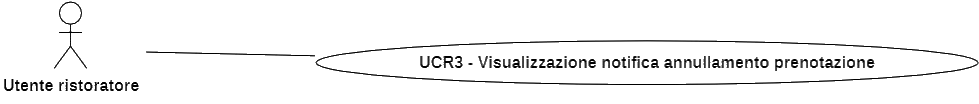
\includegraphics[width=0.9\textwidth]{./uml/UCR3.png} 
	\caption{Visualizzazione notifica annullamento prenotazione}
	\label{fig:UCR3}
  \end{figure}

\begin{itemize}
	\item \textbf{Attore principale:} Utente ristoratore.

	\item \textbf{Precondizione:} L'Utente base ha annullato la propria prenotazione (vedi \autoref{usecase:Annullamento della prenotazione}).

	\item \textbf{Postcondizione:} L'Utente ristoratore visualizza la notifica relativa all'annullamento di una prenotazione.

	\item \textbf{Scenario principale:}
	      \begin{enumerate}
		      \item Il Sistema vede che al suo interno è stata annullata una prenotazione;
		      \item Il Sistema invia all'Utente ristoratore la notifica dell'annullamento di una prenotazione;
		      \item L'Utente ristoratore visualizza la notifica relativa all'annullamento della prenotazione.
	      \end{enumerate}
\end{itemize}
